\documentclass[border=3pt]{standalone}
% Preâmbulo compartilhado pelos diagramas TikZ da aula 7 de IHR (Emoção)
\usepackage[T1]{fontenc}
\usepackage[utf8]{inputenc}
\usepackage{lmodern}
\usepackage{amsmath}
\usepackage{xcolor}
\usepackage{tikz}
\usetikzlibrary{arrows.meta,angles,quotes,decorations.pathmorphing,decorations.pathreplacing,calc,
                positioning,shapes.geometric,shapes.misc,backgrounds,fit,
                math}

% Paleta (mesma dos SVGs originais)
% Paleta da disciplina de IHR: acento azul (#1A6FB5), cor de destaque do tema.
% (o nome "dblue" é mantido para não alterar todos os diagramas)
\definecolor{dblue}{HTML}{1A6FB5}
\definecolor{dorange}{HTML}{B3541E}
\definecolor{dgreen}{HTML}{4A7C59}
\definecolor{dred}{HTML}{9C4B4B}
\definecolor{dcream}{HTML}{F4F1EA}
\definecolor{dshade}{HTML}{DDD7C9}

% Função gaussiana (não normalizada por padrão de escala visual)
\pgfmathdeclarefunction{gauss}{3}{%
  \pgfmathparse{1/(#3*sqrt(2*pi))*exp(-((#1-#2)^2)/(2*#3^2))}%
}

% Estilos comuns (prefixo d... para não colidir com chaves internas do pgf)
\tikzset{
  >={Stealth[length=2mm]},
  dguide/.style={gray!55, dashed, line width=0.4pt},
  daxis/.style={gray!60, line width=0.7pt, ->},
  dbody/.style={fill=black!3, draw=black!80, line width=1pt},
  dacc/.style={draw=dblue, line width=1pt},
  dlbl/.style={black!55, font=\small},
  dsub/.style={black!45, font=\footnotesize},
  dstate/.style={circle, draw=black!80, fill=dcream, line width=1pt,
                 minimum size=17mm, font=\large, inner sep=1pt},
  dobs/.style={circle, draw=black!80, fill=dshade, line width=1pt,
               minimum size=14mm, font=\large, inner sep=1pt},
  dbox/.style={rounded corners=2pt, draw=black!80, fill=dcream, line width=1pt,
               align=center, inner sep=6pt},
  dop/.style={circle, draw=black!80, fill=white, line width=1pt,
              minimum size=6mm, inner sep=0pt, font=\small},
  dtrans/.style={->, dblue, line width=1pt},
  dmeas/.style={->, dorange, line width=1pt},
  dcurve/.style={line width=1pt, dblue},
  dcurveb/.style={line width=1.4pt, dorange},
}

\begin{document}
\hyphenpenalty=10000 \exhyphenpenalty=10000 \tolerance=9999 \emergencystretch=3em
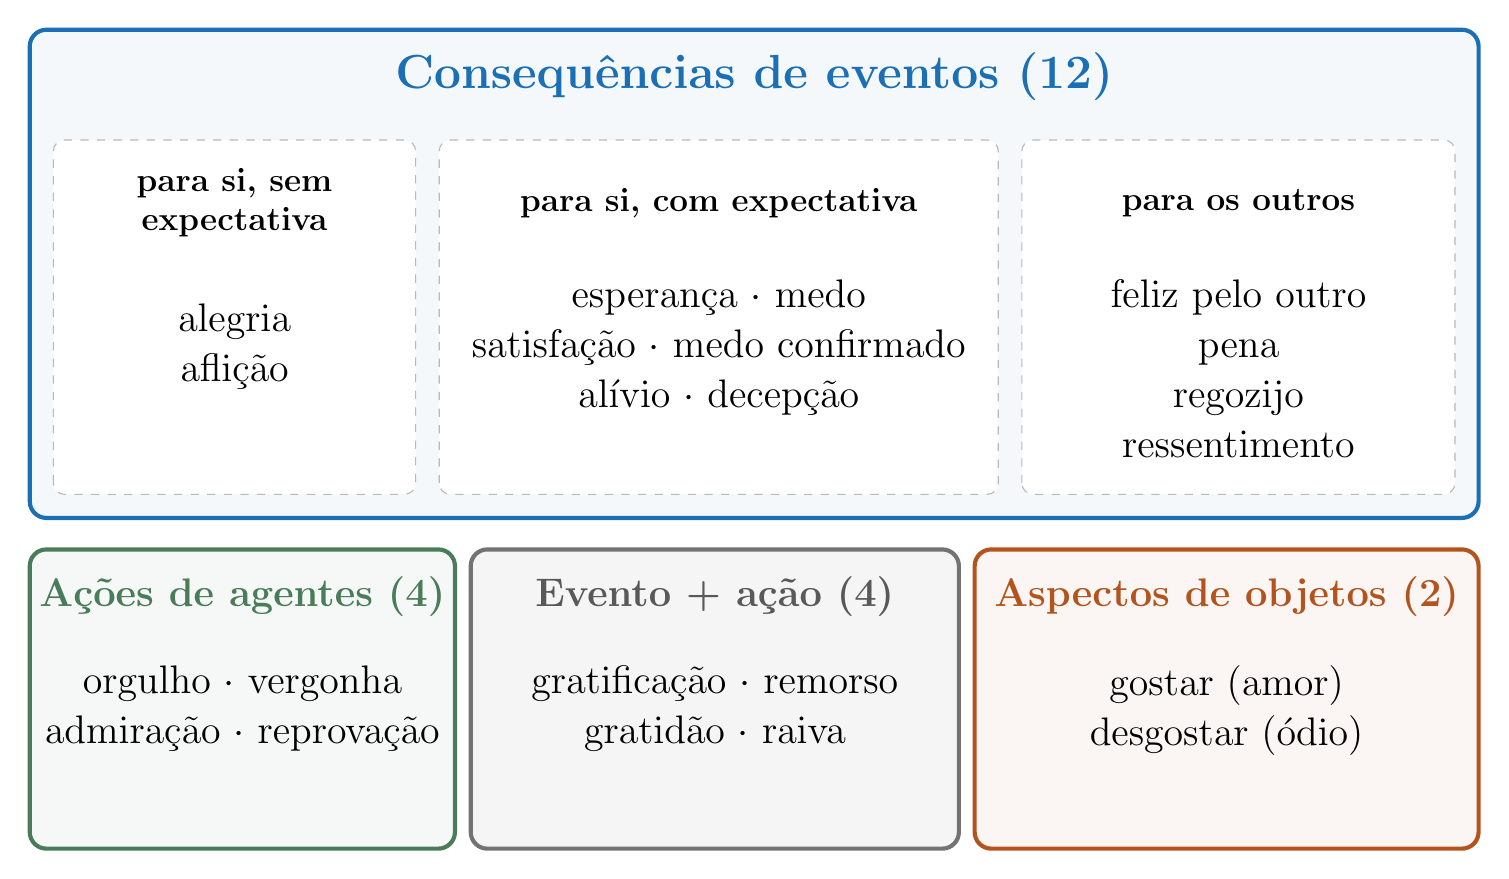
\begin{tikzpicture}[x=1cm,y=1cm]

  \tikzset{lst/.style={font=\Large, align=center, anchor=north, inner sep=2pt},
           ttl/.style={font=\large\bfseries, align=center}}

  % ===== Consequências de eventos (12) =====
  \draw[draw=dblue, line width=1.5pt, rounded corners=6pt, fill=dblue!5!white] (0,4.4) rectangle (18.4,10.6);
  \node[font=\LARGE\bfseries, dblue] at (9.2,10.0) {Consequências de eventos (12)};
  \draw[dguide, rounded corners=4pt, fill=white] (0.3,4.7) rectangle (4.9,9.2);
  \node[ttl, text width=4.2cm] at (2.6,8.4) {para si, sem expectativa};
  \node[lst] at (2.6,7.2) {alegria\\ aflição};
  \draw[dguide, rounded corners=4pt, fill=white] (5.2,4.7) rectangle (12.3,9.2);
  \node[ttl, text width=6.4cm] at (8.75,8.4) {para si, com expectativa};
  \node[lst] at (8.75,7.5) {esperança $\cdot$ medo\\ satisfação $\cdot$ medo confirmado\\ alívio $\cdot$ decepção};
  \draw[dguide, rounded corners=4pt, fill=white] (12.6,4.7) rectangle (18.1,9.2);
  \node[ttl, text width=5.0cm] at (15.35,8.4) {para os outros};
  \node[lst] at (15.35,7.5) {feliz pelo outro\\ pena\\ regozijo\\ ressentimento};

  % ===== linha de baixo =====
  \draw[draw=dgreen, line width=1.5pt, rounded corners=6pt, fill=dgreen!5!white] (0,0.2) rectangle (5.4,4.0);
  \node[font=\Large\bfseries, dgreen] at (2.7,3.4) {Ações de agentes (4)};
  \node[lst] at (2.7,2.6) {orgulho $\cdot$ vergonha\\ admiração $\cdot$ reprovação};

  \draw[draw=black!55, line width=1.5pt, rounded corners=6pt, fill=black!4] (5.6,0.2) rectangle (11.8,4.0);
  \node[font=\Large\bfseries, black!65] at (8.7,3.4) {Evento + ação (4)};
  \node[lst] at (8.7,2.6) {gratificação $\cdot$ remorso\\ gratidão $\cdot$ raiva};

  \draw[draw=dorange, line width=1.5pt, rounded corners=6pt, fill=dorange!5!white] (12.0,0.2) rectangle (18.4,4.0);
  \node[font=\Large\bfseries, dorange] at (15.2,3.4) {Aspectos de objetos (2)};
  \node[lst] at (15.2,2.6) {gostar (amor)\\ desgostar (ódio)};

\end{tikzpicture}
\end{document}
